\section{Experimental Details}
\label{app:experiments}

In this section, we provide additional details about our experiments from \cref{sec:experiments}.

\subsection{Additional Experimental Details}
\label{app:experiments:setup}

We now describe the remaining experimental details for the experiments in \cref{sec:eval:main}.

\paragraph{Coding environment}
For \planbench{} instances, we run the coding agent in a Docker container with basic tooling (python, apt-get, uv, \ldots) and Internet access.
Importantly, we remove the git commit history and all remotes.
For \swebench{}, we use the Docker images provided by~\citet{swebench}.
We let the coding agents access the web (either via dedicated tools or through the command line) and manually checked that the agents do not cheat (\eg looking at the PR corresponding to the instance description).
We find no such case of cheating, and web access represents a minority of the tool calls (less than 1\%).
For \claudecode{}, we keep the Task tool enabled: it allows \sonnet{} to invoke sub-agents, using \textsc{Haiku-4.5}, to solve sub-tasks.
For instance, a sub-task can be exploring the repository to find specific files.

\subsection{Trace Analysis}

Here, we detail the experiments from \cref{sec:eval:trace}.
In particular, we give the mapping used to aggregate tool names across coding agents, analyze the correlation between the number of tool uses and whether the tool is mentioned in the \agentsmds{}, and expand the trace analysis to the intent behind tool calls.

\paragraph{Experimental setup}
We recall the experimental setup from \cref{sec:eval:trace}.
Given a list of tool calls from an agent, we analyze the frequency of each tool call.
For tools included in the agentic framework (\eg Read, Write, or TodoWrite), we record the name of the tool being called.
For shell commands, we use an LLM to extract (from the command and its output) the concrete command that was executed (\eg \texttt{uv}, \texttt{pytest}, \texttt{cat}) and to categorize the intent of the tool call (\eg install dependencies, run tests, read files).
We build the categories iteratively.
We start with an empty set of categories, and for each shell command, we ask the LLM to assign it to an existing category if possible and otherwise create a new category.
As the LLM, we use \gptoss, and the prompt is given in \cref{app:prompts:trace_analysis}.
Finally, we manually merge duplicate and closely adjacent categories.

\begin{wraptable}[7]{r}{0.5\textwidth}
  \centering
  \vspace{-0.4in}
  \caption{Equivalence classes used to group the different tool calls.}
  \label{tab:mapping}
  \resizebox{\linewidth}{!}{%
    \begin{tabular}{lll}
      \toprule
      \claudecode{} tool & \codex{} & \qwencode{} \\
      \midrule
      Edit & \texttt{sed} & \texttt{sed}, \texttt{edit}  \\
      \midrule
      Write & \texttt{apply\_patch} & \texttt{write\_file}\\
      \midrule
      Grep & \texttt{grep}, \texttt{rg} & \texttt{grep} \\
      \midrule
      Read & \texttt{cat} & \texttt{cat}, \texttt{read\_file}, \texttt{search\_file\_content} \\
      \midrule
      TodoWrite & \texttt{update\_plan} & \texttt{todo\_write} \\

      \bottomrule
    \end{tabular}%
  }
\end{wraptable}


\paragraph{Refining the tool names}
For \cref{fig:experiment1_tool_freq}, we further manually refined the tool names for readability.
In particular, in \cref{tab:mapping}, we map tool names from other agents, namely \codex{} and \qwencode{}, as well as some CLI tools, to \claudecode{} tooling.
Lastly, for repository-specific tooling (\eg \texttt{pdm}, \texttt{ansible}, or \texttt{opshin}), we grouped them into the \texttt{repo\_tool} category. \\

\begin{figure*}[t]
    \centering
    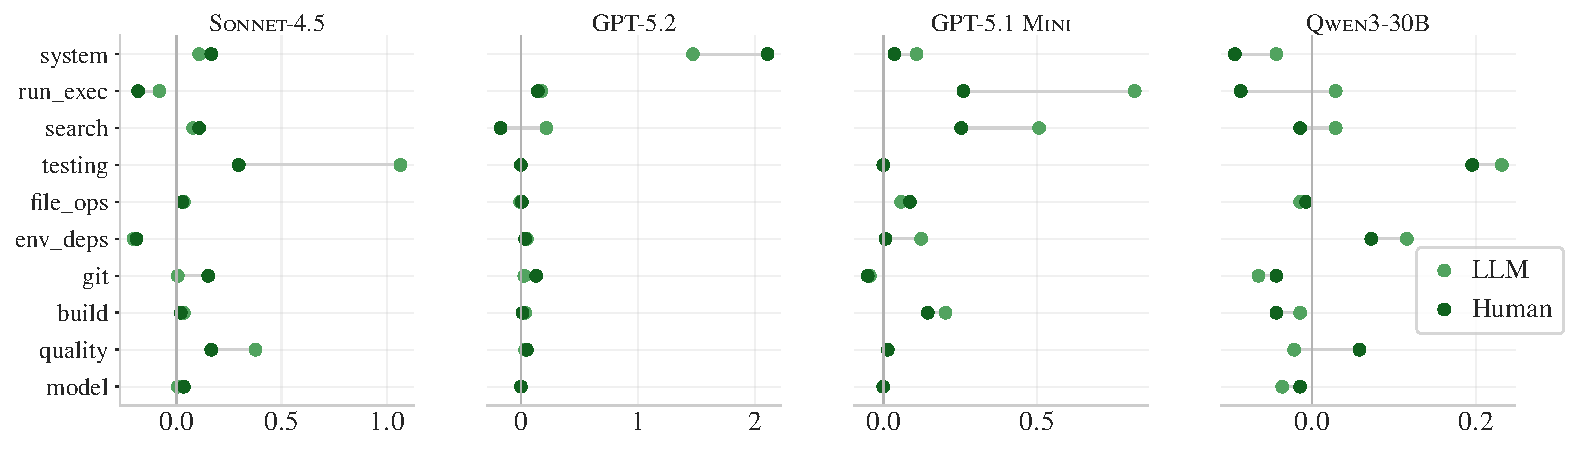
\includegraphics[width=\linewidth]{figures/appendix/trace_analysis/experiment1_toolIntent_freq.pdf}
    \caption{Increase in the average tool use (grouped into high-level categories) when including LLM-generated (bright green) or developer-provided (dark green) \agentsmds{}, compared to the average tool use without \agentsmds{}. For the high-level categories, we use an LLM to categorize the various tool calls.}
    \label{fig:experiment1_toolintent_freq}
\end{figure*}
\vspace{-0.1in}

\begin{figure*}[t]
    \centering
    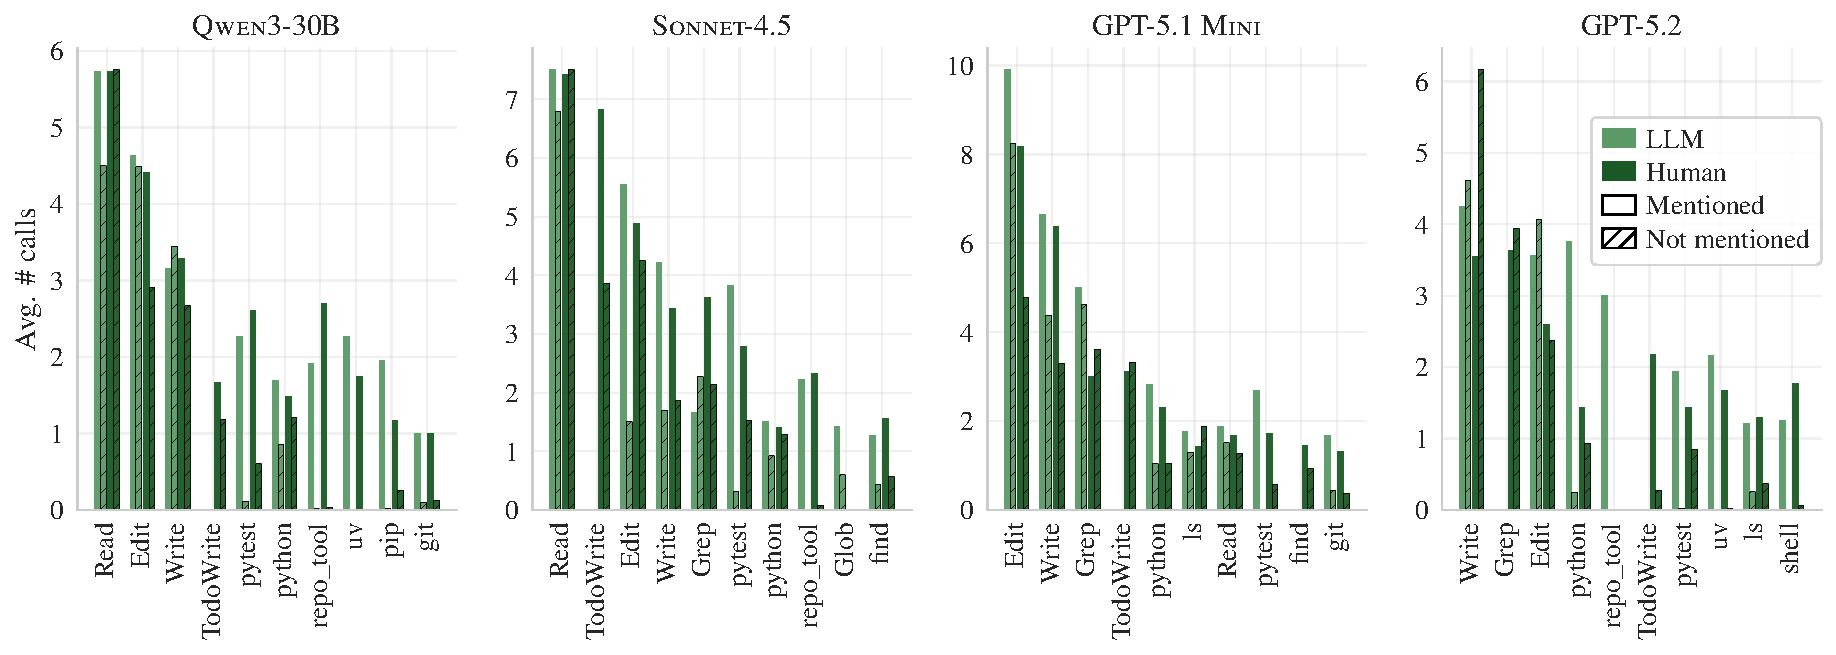
\includegraphics[width=\linewidth]{figures/appendix/correlation/tool_call_mention_correlation.pdf}
    \caption{Average number of tool calls depending on whether the tool name is mentioned in the \agentsmds{}. For tool names, we use the equivalence classes from \cref{tab:mapping}, and consider a tool to be mentioned in the \agentsmd{} if any tool from the corresponding equivalence class is mentioned in the \agentsmd{}.}
    \label{fig:experiment1_toolcall_mention_correlation}
\end{figure*}
\vspace{-0.1in}

\begin{figure*}[t]
    \centering
    \hspace*{\fill}
    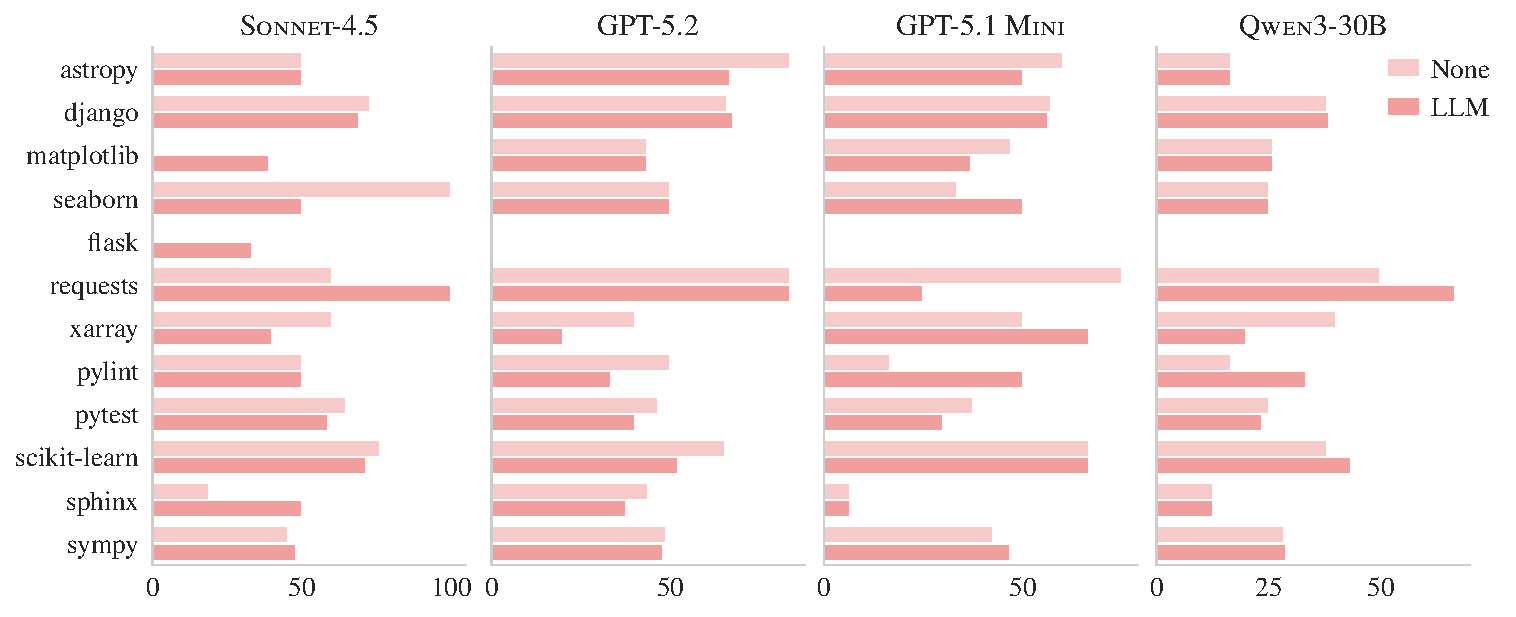
\includegraphics[width=0.97\linewidth]{figures/appendix/per_repo/experiment1_repo_accuracy_swebench.pdf}
    \hspace*{\fill}
    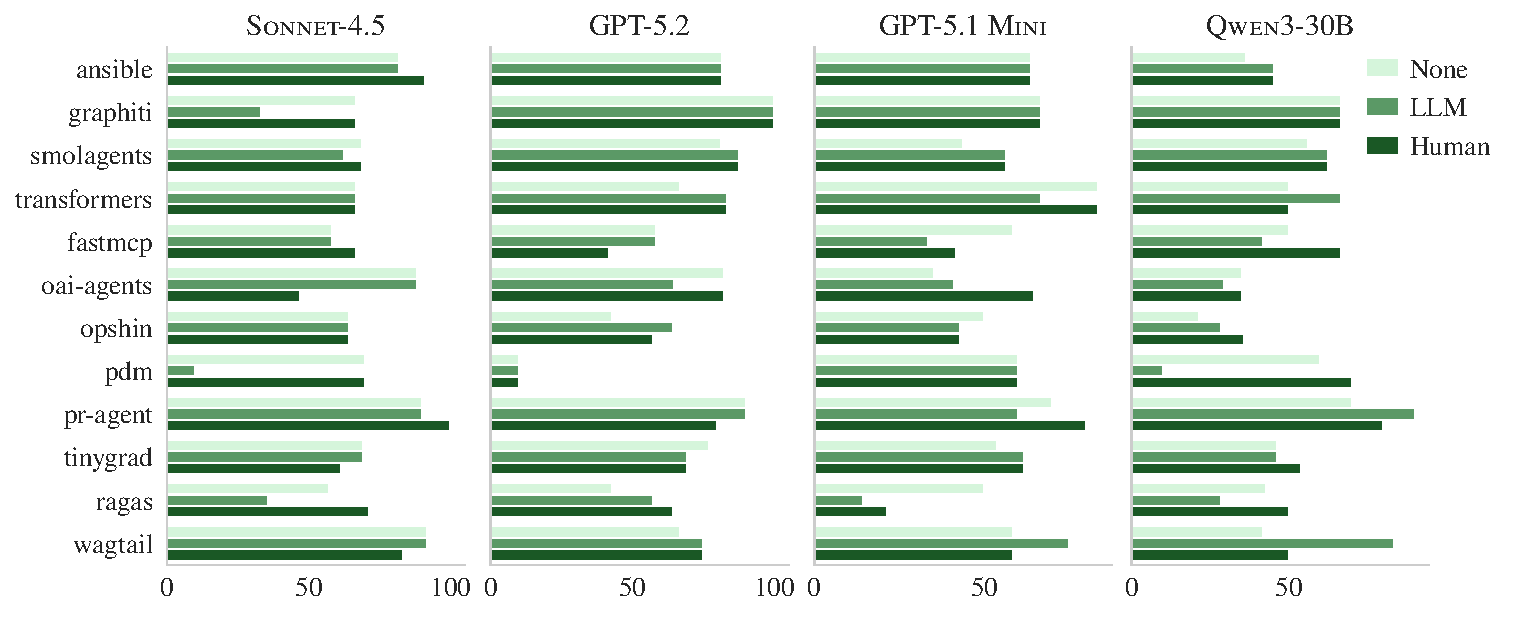
\includegraphics[width=0.97\linewidth]{figures/appendix/per_repo/experiment1_repo_accuracy_planbench.pdf}
    \hspace*{\fill}
    \caption{Resolution rate grouped by repository for four different models: without \agentsmds{}, with LLM-generated \agentsmds{}, and with developer-written \agentsmds{} on \colorbox{swebenchcolor}{\swebench{}} (top) and \colorbox{planbenchcolor}{\planbench{}} (bottom).
    For \swebench{} in particular, the majority of instances come from the same repository (\texttt{django}), making per-repository estimates of the success rate noisy.
    }
    \label{fig:experiment1_perf_pre_repo}
    \vspace{-0.15in}
\end{figure*}


\paragraph{Correlation between the number of tool calls and \agentsmds{}}
In \cref{fig:experiment1_toolcall_mention_correlation}, we show the average number of tool calls depending on whether the tool name is mentioned in the \agentsmd{}.
We find that, if a tool name is mentioned in the \agentsmds{}, this increases its usage by the coding agents.
For instance, \texttt{uv}, \texttt{pytest}, or repository-specific tools (\texttt{repo\_tool}) are used almost exclusively if they are mentioned in the \agentsmd{}.
This means that instructions in the \agentsmds{} are followed, and that a lack of instruction-following capabilities does not explain why we observe, in \cref{sec:eval:main}, no gain in accuracy when using \agentsmds{}.

\paragraph{Analyzing intents of tool calls}
For the tool intents extracted by the LLM ($334$ different categories in total), we further aggregate them into the following 10 categories:
\begin{itemize}
  \item \textbf{git}: Repository and version-control operations (e.g., commits, branches, diffs, checkout, stash, status).
  \item \textbf{model}: Model lifecycle tasks such as downloading or loading models, inspecting configurations or parameters, and running inference.
  \item \textbf{env\_deps}: Python environment and dependency management (virtualenv or venv, installations, versions, lockfiles).
  \item \textbf{build}: Building, compiling, or packaging code and producing artifacts or distribution packages.
  \item \textbf{quality}: Code quality and correctness checks (linting, formatting, type checking, validation or verification, schema checks).
  \item \textbf{testing}: Running and reviewing tests (unit, integration, regression, sanity, pytest) and test results.
  \item \textbf{run\_exec}: Executing workflows and scripts or commands (Python, shell, Django), including reproduction and debugging runs.
  \item \textbf{search}: Discovery and inspection actions (search, find, grep, glob, list, view, show, display, inspect, parse).
  \item \textbf{file\_ops}: Direct file and filesystem operations (read, write, edit, copy, move, delete, create, permissions, paths).
  \item \textbf{system}: System and miscellaneous utilities (processes, disk usage, environment variables, HTTP checks, checksums, tool or device information, help).
\end{itemize}
In \cref{fig:experiment1_toolintent_freq}, we show the difference in frequency of these categories with and without \agentsmds{}.
The conclusion is similar to that of \cref{sec:eval:trace}: the presence of \agentsmds{} significantly increases the number of tests run by coding agents, as well as the extent of codebase exploration and code quality checks.
\vspace{-0.1in}

\subsection{Per-repository Success Rate}

In \cref{fig:experiment1_perf_pre_repo}, we show the success rate of the different scenarios (\noplan{}, \autoplan{}, and \humanplan{}) grouped by repository.
For both \swebench{} and \planbench{}, there is no single repository where the presence of \agentsmds{} has a significant impact.
Nonetheless, for \planbench{} in particular, we see that the difficulty across instances is relatively balanced, validating our approach to building the instances.
\vspace{-0.1in}

